\section{Application-aware Routing}
\subsection{Application-aware Routing의 개념}
    Application-aware Routing이란 각 Application의 요구에 따라 라우팅 경로 선택 방식을 달리 하는 것이다. 오늘날 다양한 Application이 생기면서 각 Application의 요구사항 또한 다양해졌다. 고화질 동영상을 송출하는 대역폭이 중요한 Application이 있고, 실시간 영상 스트리밍과 같이 낮은 지연시간을 유지해야하는 Application이 있다. Application-aware Routing은 실시간으로 회선의 품질을 확인하여 각 Application 트래픽이 항상 최적의 경로를 이용하도록 하여 가용성을 최대화 한다. \\
    
    \vspace{-4mm}
    \begin{figure}[!h]\centering
		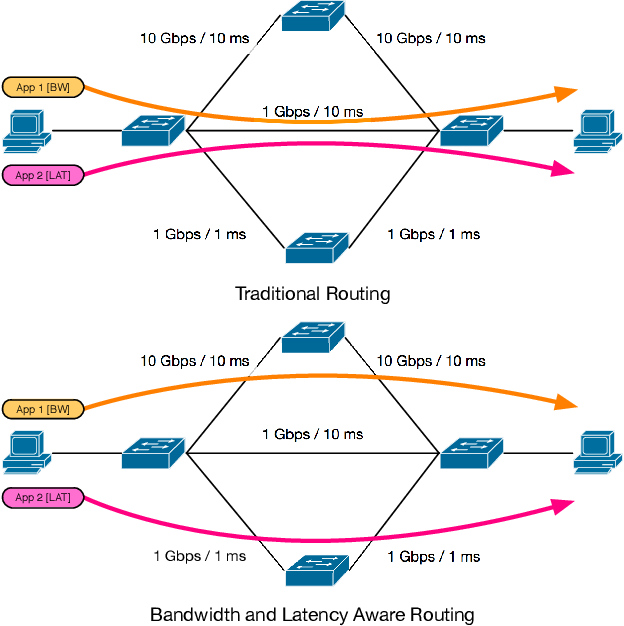
\includegraphics[width=.65\textwidth]{image/week06/5-1.png}
		\caption{\small Application-aware Routing}
		\vspace{-10pt}
    \end{figure}
    
    Application-aware Routing의 핵심은 라우터에게 Application 영역의 Data Packet 식별 능력을 부여하는 것이다. 과거의 Application들은 destination UDP/TCP port number로 식별할 수 있었다. 그러나 최근의 Application들은 대부분 HTTP/HTTPS 프로토콜을 사용하기 때문에 port number가 모두 똑같다. (HTTP/HTTPS 각각 80과 443) \\
    따라서 Application-aware Routing을 위해서 추가적인 패킷 식별 능력이 필요하다. HTTP와 같이 암호화되지 않은 패킷은 패킷 정보를 읽고 식별하기 쉽다. 하지만 HTTPS는 암호화되어 있어 패킷을 읽을 수 없고, TLS Handshake로부터 부분적인 정보를 얻어야 한다. \\
    다른 방법으로는 stream에서 pattern을 읽어서 패킷이 어떤 종류의 application의 것인지 예측하는 방법이 있다. \\
    Application 식별 메커니즘은 높은 Computational cost를 필요하기 때문에 주로 network access routers에 위치한다. SDN을 활용하면 Application 식별 메커니즘을 효율적으로 구현할 수 있다. 중심에 있는 고성능 Controller가 Computational cost가 높은 Application 식별 메커니즘을 수행하여 최적 경로를 찾아 각 OpenFlow Switch에게 전달한다. 각 OpenFlow Switch은 전달 받은 경로로 Forwarding하는 작업에 집중한다. \\
